\section{Theorie}
\label{sec:Theorie}
Ionenkristalle, wie beispielsweise CsJ, bestehen aus Kationen (Cs$^{+}$) und Anionen (J$^{-}$), welche
auf festen Gitterplätzen angeordnet sind.
Wird eine Störstelle wie ein zweiwertiges Kation, zum Beispiel Sr$^{2+}$, in den Kristall eingebaut so
entsteht eine Leerstelle an einer anderen Kationen-Stelle um die Ladungsneutralität aufrecht zu erhalten.
So entsteht ein elektrischer Dipol mit Richtung entlang der Achse der Störstellen. Dies ist in \autoref{fig:Störstelle} dargestellt.
\begin{figure}[H]
  \centering
  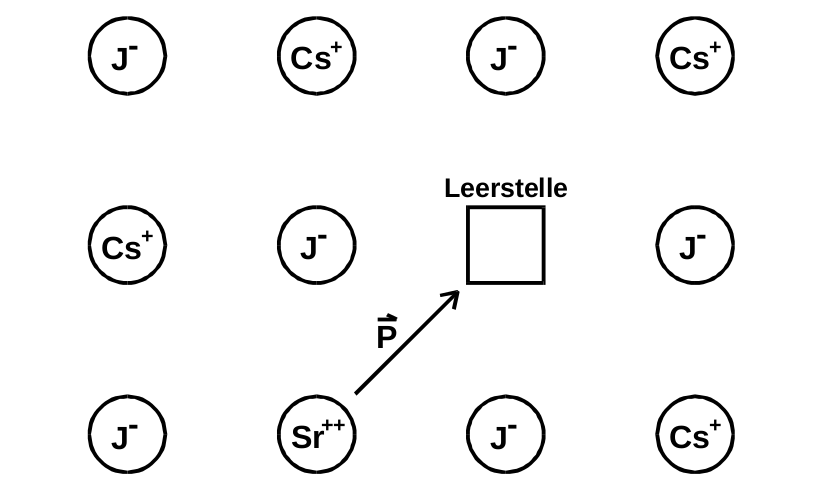
\includegraphics[width=0.6\textwidth]{pics/Stoerstelle.png}
  \caption{Schematische Darstellung eines Ionenkristalls mit einem, durch
  zwei Störstellen erzeugten, elektrischen Dipol \cite{Anleitung}.}
  \label{fig:Störstelle}
\end{figure}
Die Orientierung der Dipole sind statistisch im Raum verteilt, jedoch sind dabei auf Grund der Gitterstruktur
nur diskrete Richtungen und Beträge möglich. Eine Änderung der Richtung
kann unter einer Temperatur von 500 K nur durch Leerstellendiffusion erfolgen.
Dazu wird eine bestimmte, materialspezifische Energie $W$ benötigt, um das Gitterpotential zu überwinden.
Die Anzahl der Dipole mit einer ausreichend großen thermischen Energie folgt der Boltzmann-Statistik.
Ebenso folgt die mittlere Zeit zwischen zwei Umorientierungen, die Relaxationszeit $\tau$, dieser Verteilung.
\begin{equation}
  \tau(T) = \tau_0 \exp{\left(\frac{W}{kT}\right)}
  \label{eq:Relaxationszeit}
\end{equation}
Dabei ist $\tau_0$ die charakteristische Relaxationszeit.\\
Wird der Kristall in ein elektrisches Feld gebracht richtet sich ein Teil $y$ der Dipole in Richtung
des Feldes aus. Dieser wird durch die Langevin-Funktion
\begin{equation}
  y = L\left( \frac{pE}{kT}\right) = \coth{\left( \frac{pE}{kT}\right) - \frac{kT}{pE}}
\end{equation}
beschrieben, welche für $pE \ll kT$ mit
\begin{equation}
  y(T)=\frac{pE}{3kT}
\end{equation}
genähert werden kann.
Da die Relaxation thermisch bedingt ist, lässt sich die Ausrichtung bei tiefen Temperaturen
einfrieren.
Da \autoref{eq:Relaxationszeit} Temperaturabhängig ist, richten sich die Dipole bei zunehmender Temperatur
wieder nach einer statistischen Verteilung aus.
